\chapter{Operational parameter exploration and their implications}

\section{Introduction}

Building on the foundations laid by the preceding chapters, this chapter delves into a more nuanced investigation of the parametric influences on the resulting force curves obtained through Atomic Force Microscopy (AFM). When operating an AFM, it is typical to use a standard set of operational parameters. \cite{Schirmeisen2007} These parameters are often found during operation in an exploratory manner to find a good signal to noise ratio. However, it can be prudent  to examine a spectrum of force curves under varied conditions, aka a sensitivity analysis. Such an investigation enables the assessment of result consistency across diverse settings, thereby ensuring that the observed outcomes are not merely artifacts of parameter-specific minima phenomena. Additionally, a range of differing conditions can provide an insight into how other phenomena may have an effect on the observed behaviour of the curves.

A range of differing conditions were repeated with the following parameter changes: Tip speed, dwell time, solution pH and force mapping. 

\subsubsection{Tip Speed Variations}
The velocity of the AFM tip's approach and retraction impacts the force measurements, potentially altering the energy landscape of particle interactions. Varying the tip speed not only affects the kinetic parameters but also provides insight into time-dependent phenomena such as lubrication forces and simple viscous drag. The adjustment of the tip's velocity probes the dynamic response of the system, shedding light on the viscoelastic properties of the medium and the rate-dependent behavior of interparticle forces.

The previous results were taken at 0.5 Hz, or a tip speed of 1 $\mu$m/s. Two other speeds were used; 0.1 Hz (0.2$\mu$m/s) and 2 Hz (4$\mu$m/s). 0.1 Hz was used exclusively for 10 mM.

\subsubsection{Effect of Dwell Time}

The incorporation of a 5-second dwell time between the approach and retraction phases is intended to allow the system to relax and achieve a more stable equilibrium state. This pause in movement is designed to mitigate the effects of transient forces that might arise during rapid measurements, thereby enabling the detection of more subtle, time-dependent interactions that might otherwise be overlooked. The dwell time enhances the visibility of forces that develop more gradually, such as those influenced by the restructuring of the solvation shell around the interacting surfaces. Additionally, it could amplify the observation of hydration forces and the formation of solvation layers. These phenomena are typically more pronounced under conditions where the interacting surfaces have sufficient time to stabilize within the liquid environment. 

\subsubsection{Solution pH Influence}

The pH of the solution influences the surface charge on the silica particle tip, which, in turn, modulates the observed force interactions. Variations in pH are expected to alter the electrical double layer, thereby affecting the force profiles and interaction potentials. 

\subsubsection{Forcemapping for wide range site analysis}

Forcemapping, a method of tracking force-distance curves over a defined grid area, was employed to obtain a comprehensive understanding of the force distribution across the sample. This technique is useful in discerning how heterogenious the analysed surface is and provides data that could allow for a statistical analysis of interparticle forces across a range of areas.

The exploration of these parameters serves not just as a methodical inquiry into the forces acting within colloidal dispersions, but also as a means to justify our approach to force curve analysis. The diversity of these conditions reflects the complex nature of the studied system and underscores the need for a comprehensive dataset that accurately represents the multifaceted nature of particle interactions.

The subsequent section presents the force distributions across our dataset, providing empirical evidence for the impact of these parameters. Finally, the section highlights the differences between the ``standard" dataset and the modified parameters.

\section{Tip speed analysis}

One of the differences between the different tip speeds was the data density. For faster speed less data was taken, while slower speeds had more data taken. This was due to the rate in which the AFM takes in data - the AFM was set to take in the maximum rate of data throughout the whole process. This was done to maximise the volume of data usable for the binning process (as seen in chapter 5). 

For 0.1 and 0.5Hz frequencies, the data recording rate was sufficient to the support the processing of the curves, while 2Hz had significantly less data volume, and required more involved operator tuning, with generally a lower bin size setting used in the script. As each bin contained less data, the background noise was more dominant in the data, increasing the noise in the resulting averaged curve. 

For each of the points, the tip speed increase was done after the initial reading, thus meaning that the sites can be directly compared across the standard dataset and this dataset (i.e. 0.5Hz dataset was recorded, then 2Hz was recorded right after in the same area).

Due to the lower data density and the force cap set at around 12 nN, there was a smaller range of data points in which to fit the contact region when compared to 0.5 Hz, leading to a higher failure rate by the script for each movement. It is important to highlight that for this concentration, the retract force histogram shows no attractive force associated with the return movement. This absence could suggest that the higher speeds used in this experiment did not allow the system sufficient time to relax towards an attractive profile. Alternatively, this could indicate that the decay of the electrostatic component is time-dependent, requiring more time to establish or dissipate than was permitted by the experimental conditions, as explained below.

\subsection{Expected effect of tip speed on results}

As ions redistribute themselves, they can more effectively screen the surface charges, which reduces the electrostatic repulsion. At slower speeds (0.1 Hz), these ions have more time in order to arrange themselves, and therefore reduce the strength of the electrostatic repulsion. This screening effect means that the repulsive force might be weaker than what would be observed if the ions were not given time to arrange themselves.

At higher speeds (2 Hz), the faster approach does not give ions sufficient time to rearrange and fully screen the surface charges. This incomplete ion distribution can lead to less effective screening and therefore a stronger observed electrostatic repulsion compared to slower approaches.

The force applied to the tip can be calculated using Stokes' law given in \ref{eqn:Stokesdrag}. \cite{bird2001transport}

The dynamic viscosity was calculated to be 0.0069 $Ns/m^2$ for 50:50 water:glycerol. \cite{Viscosity1} \cite{Viscosity2} Using this equation, the following expected force applied to the cantilever: $4.2e^{-14}$ N, 0.5Hz: $2.1e^{-13}$ N, 2Hz: $1.7e^{-12}$ N. Given the smaller magnitude it is expected that the change in tip speed shouldn't influence the results, or, the influence of tip speed is unlikely to be due to hydrodynamic forces in this case.

\subsubsection{Averaged curve of data}

Force curves were taken for each concentration, and processed in the same way as Chapter 5 for the approach curve, and chapter 6 for the retract curve using the script detailed in Chapter 4. These datapoints were then averaged, with the standard deviations ($Stdev_{avg}$) calculated between sites using equation \ref{eq:Stdevavg}

These points were then plotted against the original dataset to investigate if any noticeable overall differences between points could be discerned.

\begin{figure}[h!]
\centering
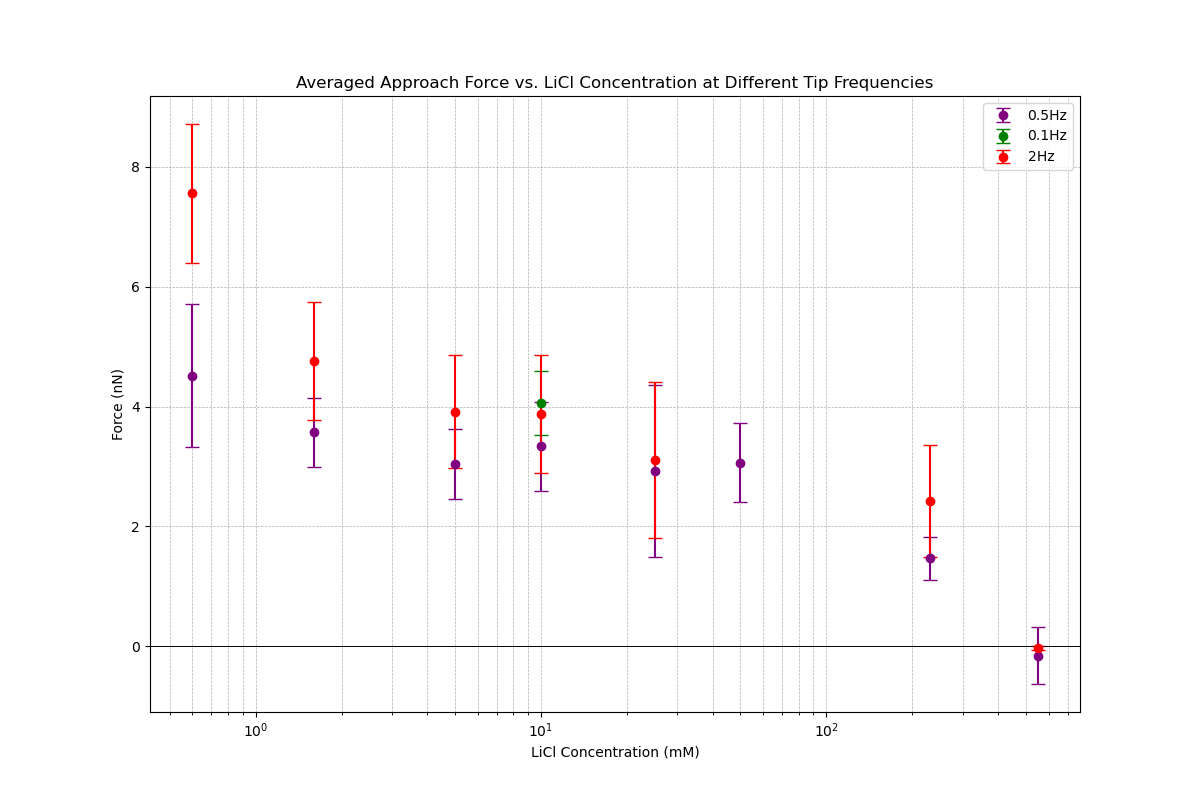
\includegraphics[width=\textwidth]{chapter7/Tip speed/Overall graph approach.png}
\caption{Averaged approach curve with the range of tip speeds. 0.5Hz represents the standard dataset, whereas 0.1Hz and 2Hz represent the modified speeds under investigation.}
\label{fig:ApproachAverageSpeed}
\end{figure}

The approach curve (Figure \ref{fig:ApproachAverageSpeed}) demonstrates an interesting observation: While minor, the increase in tip speed seems to indicate that the force required to bring the tip in contact increases with the speed of the tip. Possibly indicating that the system relaxes or changes in response to an approaching surface. 0.6mM is particularly interesting - as there was a significant increase in repulsive force at the higher speed, potentially indicating that tip speed has larger effects at very low ionic concentrations. 550mM is also interesting, where there was very little in the way of variation, and the approach force was nearly 0, potentially indicating that as the tip approaches, the surface was unable to relax in this way. 0.1Hz, while interestingly overlaps with the 2Hz datapoint, does not represent enough datapoints to fully make any solid conclusions. 

demonstrates an interesting observation: while minor, the increase in tip speed seems to indicate that the force required to bring the tip in contact increases with the speed of the tip. This observation could suggest that the system does not have sufficient time to relax or equilibrate as the surface approaches, potentially due to the rapid movement reducing the time for ions to rearrange and screen the electrostatic forces effectively.

For the 0.6 mM concentration, a significant increase in repulsive force was observed at higher speeds. This finding indicates that the speed of the tip may have a more pronounced effect at very low ionic concentrations, where the electrostatic forces are more dominant, and any disturbance in the ion distribution could significantly impact the observed force.

In contrast, at 550 mM, the variation in approach force was minimal, with the force nearly approaching zero. This could suggest that at higher ionic concentrations, the system reaches a state where the ions effectively screen the electrostatic forces, and the surface interactions become less dependent on the approach speed.

The overlap of the 0.1 Hz data with the 2 Hz data point suggests that at this lower speed, the system might have had enough time to relax or that other interactions, such as hydrodynamic forces, became more significant. However, the limited number of data points at 0.1 Hz prevents drawing solid conclusions from this observation.

\begin{figure}[h!]
\centering
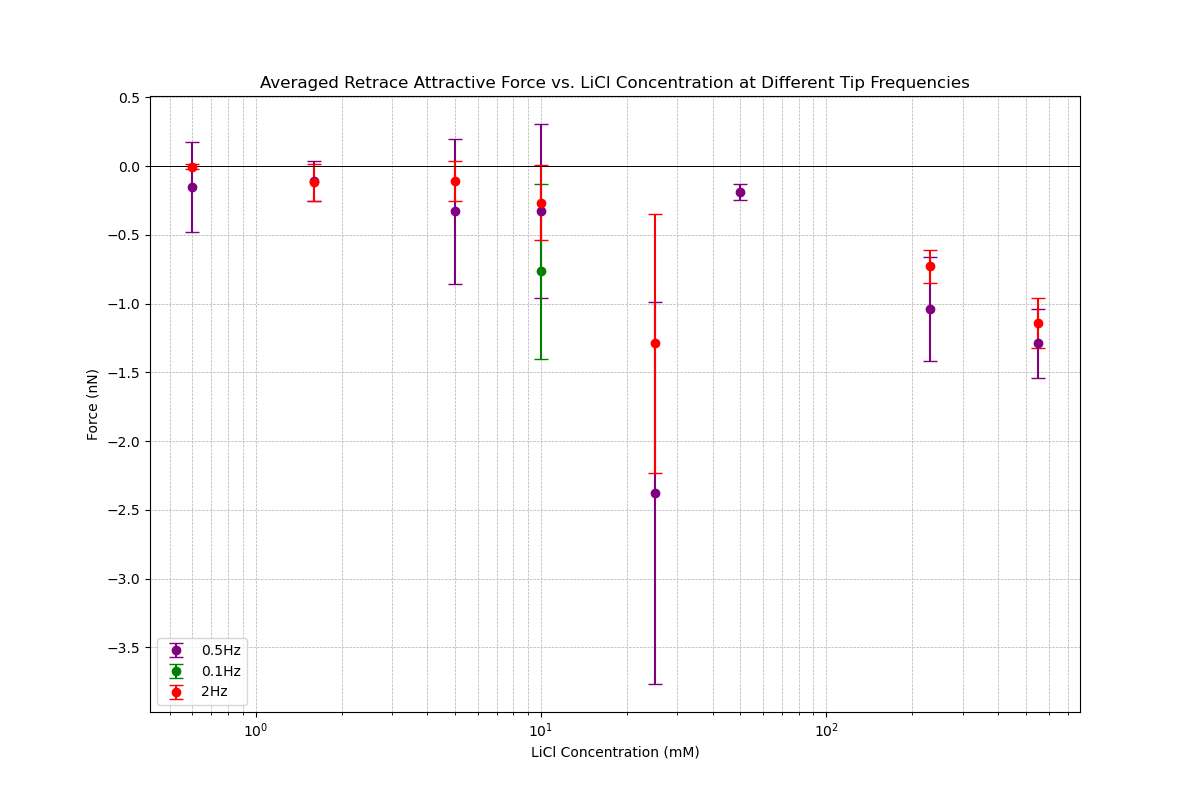
\includegraphics[width=\textwidth]{chapter7/Tip speed/Overall graph retrace.png}
\caption{Averaged retract curve with the range of tip speeds. 0.5Hz represents the standard dataset.}
\label{fig:RetractAverageSpeed}
\end{figure}

The retrace curve (Figure \ref{fig:RetractAverageSpeed} shows a similar story - 
during the majority of retraction phases, the AFM tip encounters less attraction to the surface, making disengagement easier. This observation suggests that under specific conditions, the system may undergo a relaxation process, thereby diminishing the attraction during retraction. Notably, at a 0.6 mM concentration, there is no substantial variation observed in the retraction phase compared to the approach, with values remaining within expected ranges. This implies that slower tip speeds might enhance the attractive interaction between the tip and the surface. Additionally, an intriguing observation is made with the 25 mM data points; despite the reduced range and magnitude of the attractive force spike in the data, the consistency across different speeds suggests that the effect is more likely due to site-specific factors rather than speed variations. This is further corroborated by findings in Chapters 5 and 6, where 25 mM data were hypothesized to result from either tip or solution contamination.

Another aspect of investigation worth looking into is how the speed influences the reliability of the data. As tip speed increases, the volume of data decreases, as mentioned before, and as such it stands to reason that the standard deviation of the data would increase with this phenomena too.

\begin{figure}[h!]
\centering
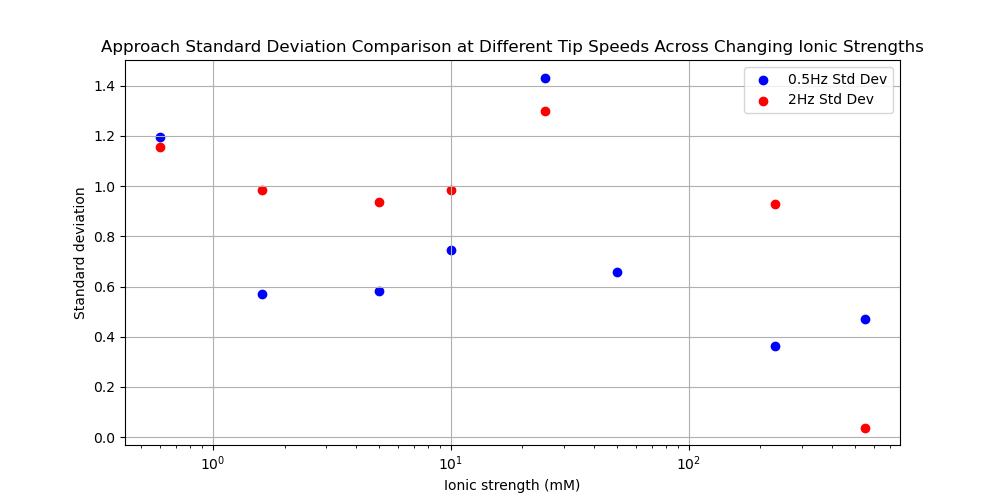
\includegraphics[width=\textwidth]{chapter7/Tip speed/Standard deviation change.png}
\caption{Averaged approach standard deviation between points. 0.5Hz represents the standard dataset.}
\label{fig:ApproachAverageSpeedDev}
\end{figure}

For the majority of the data points, the general observation holds true ($Figure \ref{fig:ApproachAverageSpeedDev}$, with 0.6 mM and 25 mM concentrations slightly below the slower value. However, the 550 mM data point stands out as an exception. 


\begin{figure}[h!!!]
\centering
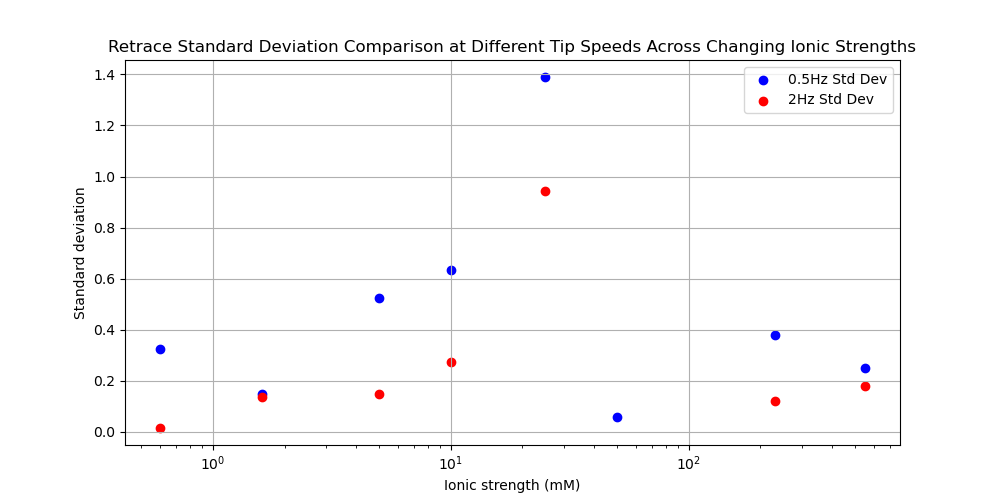
\includegraphics[width=\textwidth]{chapter7/Tip speed/Standard deviation change retract.png}
\caption{Averaged retract standard deviation between points. 0.5Hz represents the standard dataset.}
\label{fig:RetractAverageSpeedDev}
\end{figure}

When examining the retract curve (Figure \ref{fig:RetractAverageSpeedDev}), our expectations are reversed. For each of the data points, there is less variation between points, suggesting that a faster tip speed results in a more stable analysis for the retraction phase. This finding could support the idea that with less time for the system to relax and adapt, the retract phase provides more consistent results in a less variable environment.

The other question that is raised by this analysis is thus, if a tip is held in constant contact and allowed to relax, how would that affect the results? This leads us directly into our next section, the dwell time analysis.

\section{Dwell time}

The dwell time represents the time in which the tip is held down onto the surface between the approach and retrace curves. This is usually done by the system attempting to use the feedback mechanism to keep the force applied to the tip at a constant force. This action was done for each and every curve taken on the machine for the dwell dataset.

For this series of data, only one point per concentration was done. This was due to the increased strain this often puts on the cantilever, which was an important and managed resource throughout this investigation. Overindulgence in certain aspects of the experimental protocol may lead to underindulgence or lack of exploration in other areas. As a result, a series of repeats could be performed to improve this analysis. For this case, the single dwell datapoints were compared against the averaged standard dataset points.

One other frustration seen during this operational mode was the inconsistency in data shape. This made using the analysis software particularly challenging, and is an area of potential improvement for the script. The script expects the user to provide a clear series of data with an approach and retrace aspect separated clearly, however, due to the 5 second dwell time providing a high degree of variability in forces, this can often trip up the detection method used to differentiate between the two phases. While two datapoints where successfully analysed using the script (25mM and 230mM) the other datapoints would've required a significant rewrite. As such, a simplified script was written to extract the peak force from the retrace curve, as, in theory, the only portion of the curve affected should be the retrace due to the potential impact of dwelling only being felt during the retrace curve.

\begin{figure}[h!]
\centering
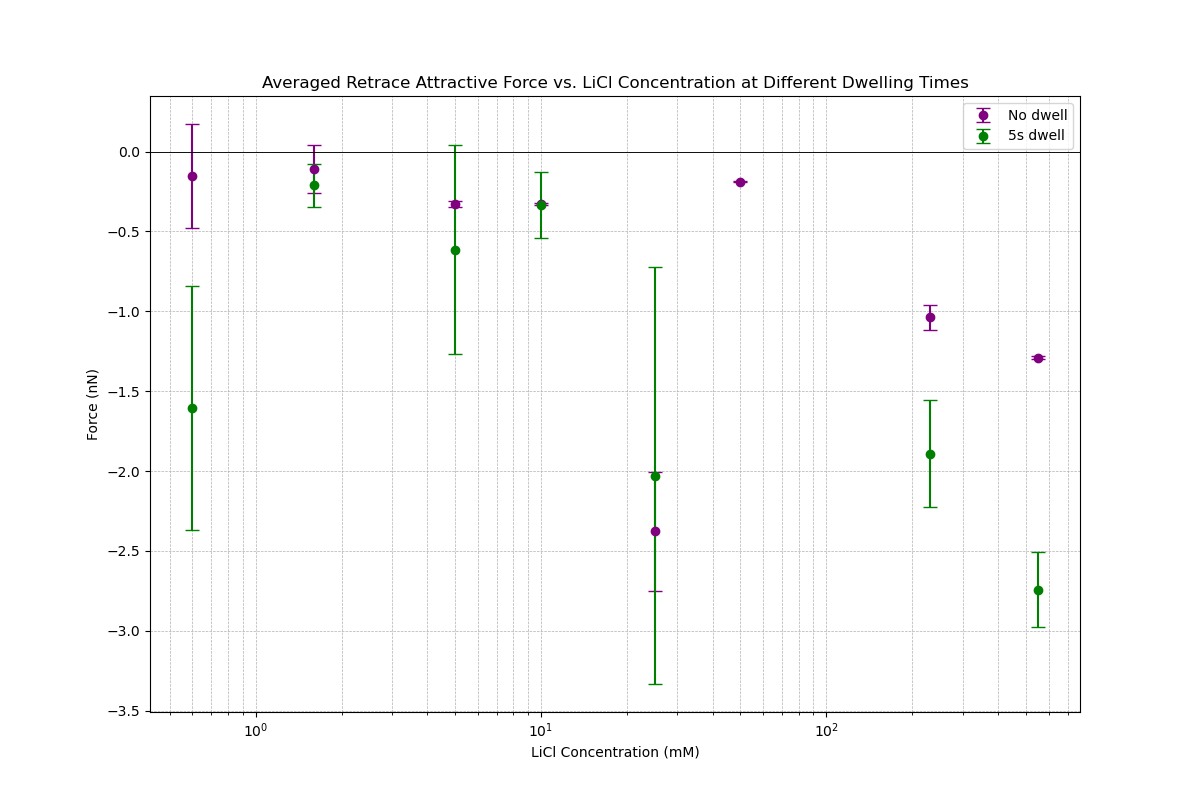
\includegraphics[width=\textwidth]{chapter7/Dwell/Retrace overall.png}
\caption{A graph demonstrating the averaged retract forces felt by the AFM tip at different LiCl concentrations with 5s dwell time and 0s dwell time respectively.}
\label{fig:RetractDwell}
\end{figure}

The retrace curve presents (Figure \ref{fig:RetractDwell}) an interesting but not unexpected conclusion: Aas the tip exposure time increases, the retentive force between the surface and tip also increases during the retrace motion, particularly for the 0.6 mM, 230 mM, and 550 mM data points. However, the data for 25 mM stands out, as it shows an inverse relationship where the retentive force decreases. This could be due to the previously discussed relaxation time or due to the previously discussed contamination explanation in prior chapters.

\begin{figure}[h!]
\centering
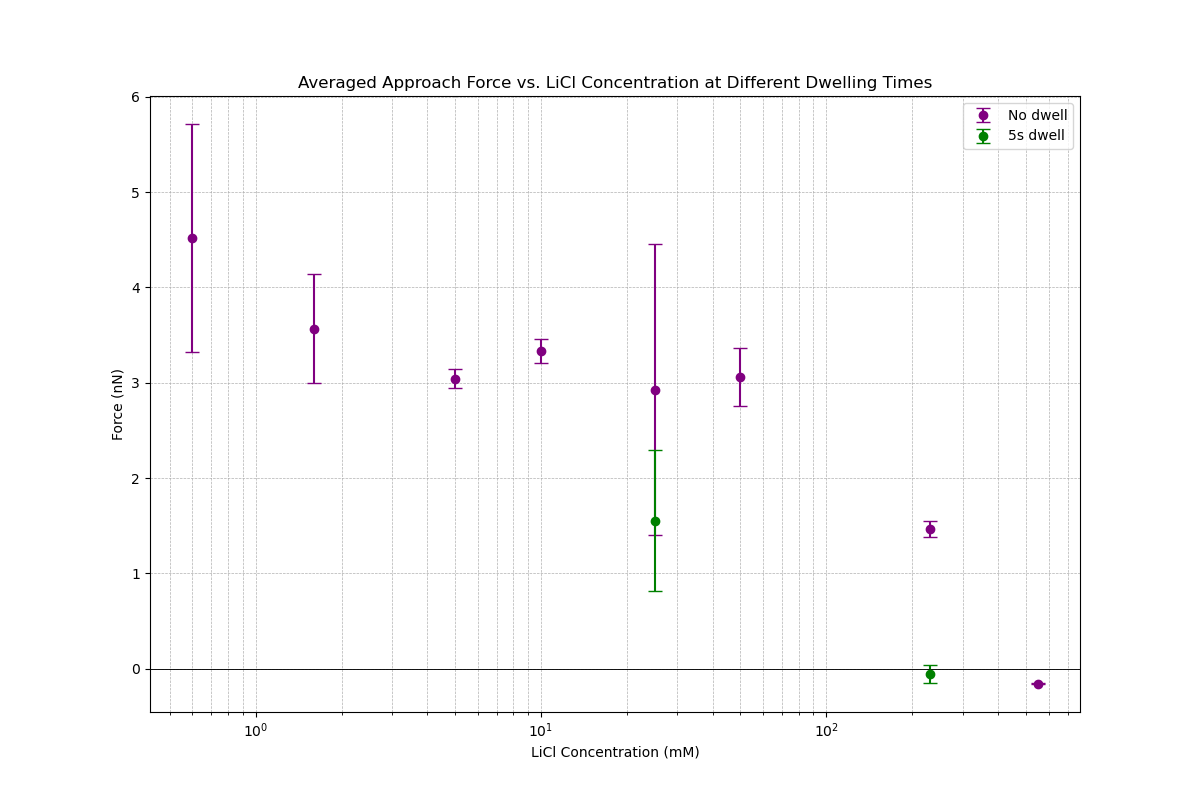
\includegraphics[width=0.95\textwidth]{chapter7/Dwell/Approach overall.png}
\caption{A graph demonstrating the averaged approach forces felt by the AFM tip at different LiCl concentrations with 5s dwell time and 0s dwell time respectively.}
\label{fig:ApproachDwell}
\end{figure}

However, when we look at the approach curve for the 2 dwell points (figure \ref{fig:ApproachDwell}, we see an interesting picture. As the dwell time increases, the time between consecutive curves also increases, allowing more time for water molecules and ions to reorient and adapt to the approaching tip, leading to a decrease in the observed repulsive force. This suggests that hysteresis effects might play a significant role in the interaction dynamics.

\newpage
\section{pH analysis}

The pH of a solution can significantly affect the forces between silica particles in a 50:50 water-glycerol solution due to changes in the surface charge of the silica interfaces. At different pH levels, the degree of ionization of silanol groups on the silica surface can vary, which impacts the electrostatic component of the total interparticle force. 

Silica surfaces are known to have silanol groups that can either accept or donate protons depending on the pH. At pH 5, which is close to the isoelectric point of silica, the surface charge density is reduced. This condition is interesting for force measurements since the electrostatic repulsion between particles is minimized, allowing other forces (such as van der Waals or steric forces) to be more prominently observed. \cite{Pavan2019}

While the solutions used in the standard dataset was around pH 7 on creation the pH can drift to slightly acidic due to carbon dioxide (CO\textsubscript{2}) from the air dissolving in the water, forming carbonic acid (H\textsubscript{2}CO\textsubscript{3}), which can dissociate to form bicarbonate (HCO\textsubscript{3}\textsuperscript{-}) and hydrogen ions (H\textsuperscript{+}). Though this effect is generally quite small, it is worth investigating to see if changes in pH could've altered the resulting dataset.

For this analysis a solution made up to pH of 5 instead of the standard pH 7 was performed, with the results directly compared against the 0.6 mM LiCl concentration solution. 

\begin{figure}[h!]
\centering
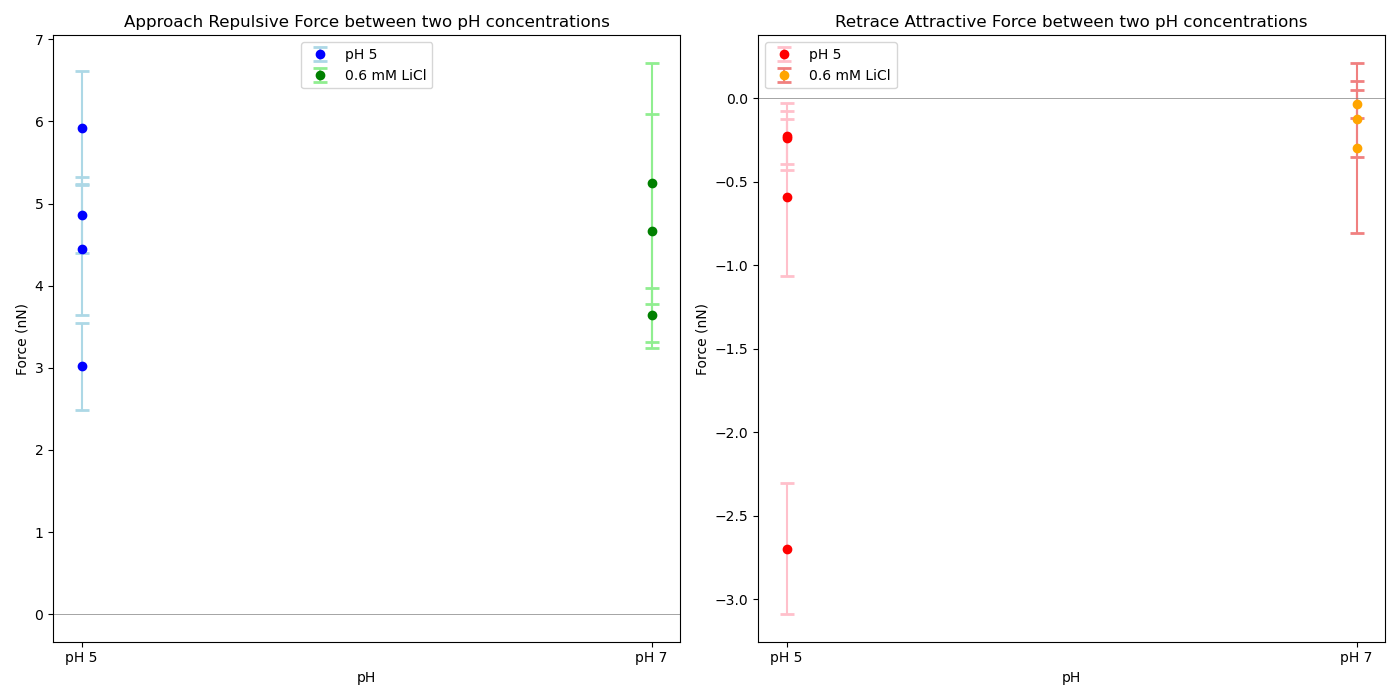
\includegraphics[width=\textwidth]{chapter7/pH/Overall image.png}
\caption{A graph demonstrating the differences in approach and retract forces at differing pHes. pH 5 is the deviation and pH 7 is the standard.}
\label{fig:pHOverall}
\end{figure}

From the observed change in pH, the resulting forces are similar to what would be expected with a pH 7 enviroment (0.6 mM LiCl), with a striking overlap between the two data series on approach. The only observable difference between the two is in the retrace curve, where one site expresses significantly more attraction.


\newpage
\section{JPK Forcemapping}

One of the limitations of using the interpretation software is that it assumes that all curves are of the same shape. This is not the case for a range of sites. While this helps highlight features (such as the shelf) across multiple repeats on the same area, it does not take into account a range of different sites. That being said, however, as long as the user does not attempt to use the software incorrectly to provide an averaged graph, the attractive/repulsive force analysis is perfectly applicable and as such was used to analyse each induvidual curve from the forcemapping.

Due to the differences between the AFMs, and potentially the way the AFMs were used to measure the interactions, the ``shelf" seen was more of a snap to contact point in the curve. This meant that the shelf seen in the previous AFM, may have been the point in which the tip snapped to the surface, and the older AFM may not have been able to detect or measure this sudden change in the way the new one has. 

This may be due to the rate in which the data is collected, or differences in how the cantilever is physically handled. If a snap to contact is only observed by the data points around either side of the event, the resulting curve will indicate that it is flat. However, in Chapter 8, an example curve is given, showing that the snap to contact physically brings the cantilever down into contact with the surface (figure \ref{fig:noisey}). 

Due to the limited window in which this AFM was available, it was not possible to explore this interaction further, but it is promising that this shelf feature is present across multiple AFMs and sites. The script was adapted in order to use the new data type, with a specialised script written to convert exportable JPK filetypes into the format expected by the software.

The operation of the AFM was done with the same tip and conditions, with a 16x16 grid with a 1 \textmu m distance between each of the sites. Only 2 concentration could be performed during the available time: 0.6 mM and 10 mM. For each grid a histogram was created to display the range of forces across the entire scan.

\subsubsection{0.6mM approach}

As the script is written to concatenate a range of graphs into a single one, there were some quirks of processing. For one, the histogram shows a range of forces, but it is important to know that for this range it is across different areas of the glass, rather than a single area.

% Approach f c hist
\begin{figure}[h]
    \centering
    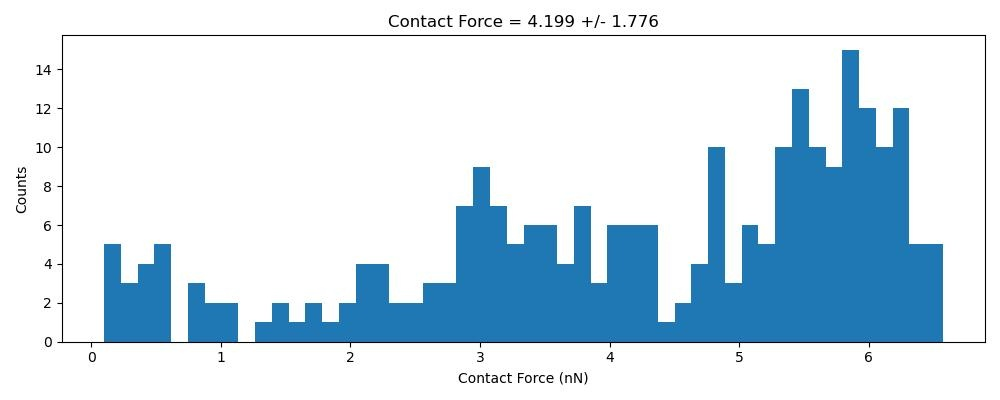
\includegraphics[width=0.8\textwidth]{chapter7/ForceMaps/0.5mM/approach_f_c_hist.jpg}
    \caption{Approach force histogram for 0.6 mM concentration.}
    \label{fig:approach_f_c_hist_0.5mM}
\end{figure}

% Approach df zp bin
%\begin{figure}[h]
%    \centering
%    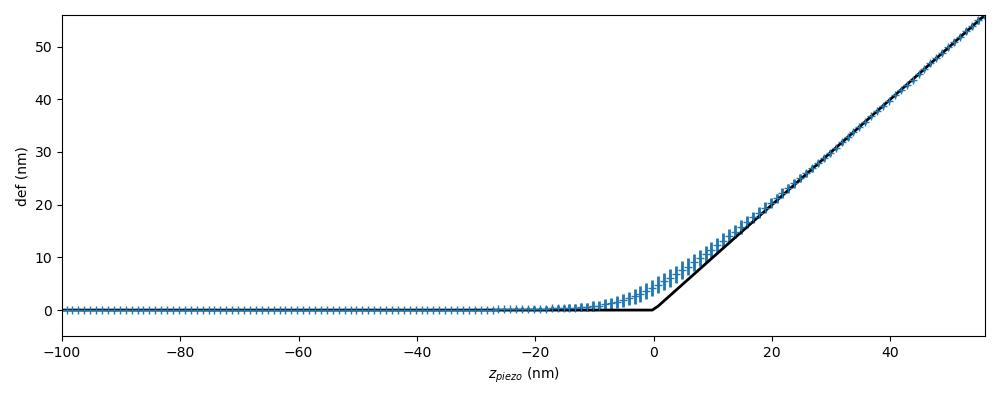
\includegraphics[width=\textwidth]{chapter7/ForceMaps/0.5mM/approach_df_zp_bin.jpg}
%    \caption{Approach df zp bin for 0.5mM concentration.}
%    \label{fig:approach_df_zp_bin_0.5mM}
%\end{figure}

% Approach heatmap
\begin{figure}[h]
    \centering
    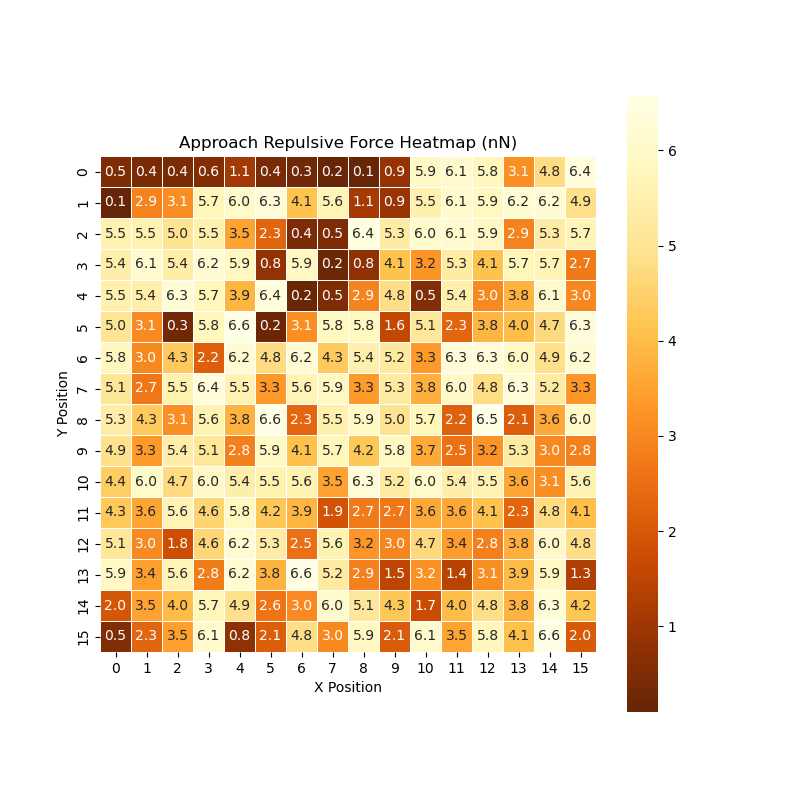
\includegraphics[width=\textwidth]{chapter7/ForceMaps/0.5mM/Approach heatmap.png}
    \caption{Approach heatmap for 0.6mM concentration.}
    \label{fig:approach_heatmap_0.5mM}
\end{figure}

The heatmap demonstrates the wide range of variability seen on a glass surface. This indicates that interacting surfaces is significantly dependent on local conditions of the surface. A range of forces is present, indicating variability in the interaction forces across different points on the surface. This could be due to surface heterogeneities or variations in local chemical composition and structure. 
\newpage

\subsubsection{0.6mM retract}

For the retraction portion of the curve, the histogram shows the distribution of attractive forces measured during the retract phase across all different sites. Most measurements cluster around a relatively small attractive force as seen in the standard dataset, but there is an outlier showing a strong attraction. This suggests that while the retract forces are generally consistent, certain specific interactions result in much stronger attraction. This could be due to a contaminant on the surface, or a significant surface profile feature (roughness).

% Retract f a hist
\begin{figure}[h!!!]
    \centering
    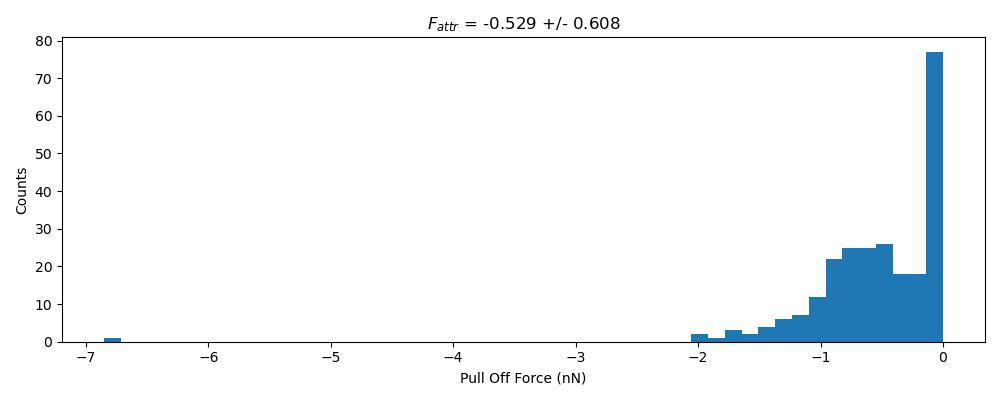
\includegraphics[width=0.8\textwidth]{chapter7/ForceMaps/0.5mM/retract_f_a_hist.jpg}
    \caption{Retract force histogram for 0.6 mM concentration.}
    \label{fig:retract_f_a_hist_0.5mM}
\end{figure}

% Retract heatmap
\begin{figure}[h!!!]
    \centering
    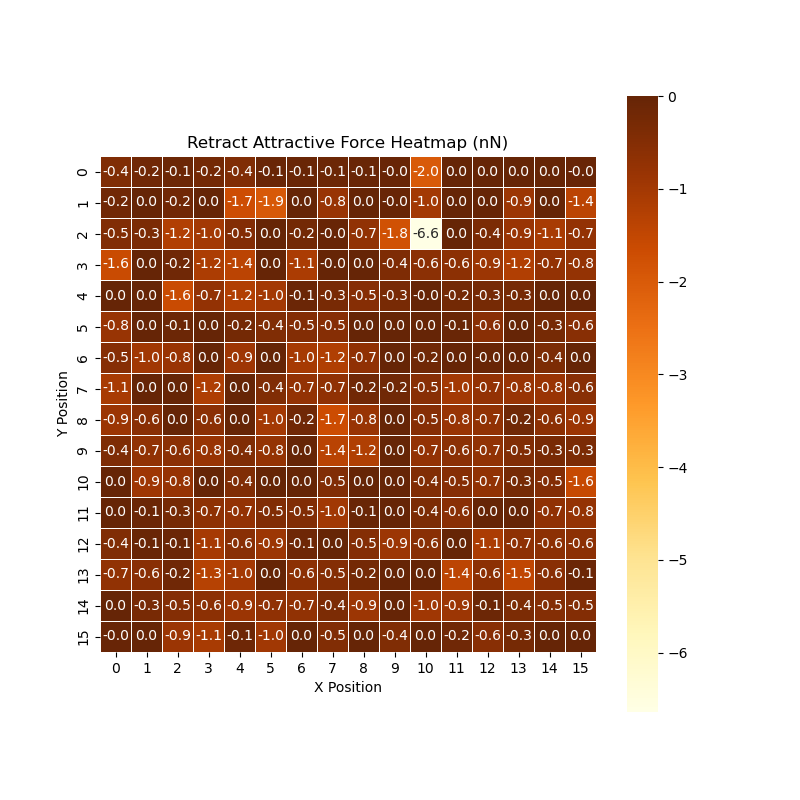
\includegraphics[width=0.8\textwidth]{chapter7/ForceMaps/0.5mM/Retract heatmap.png}
    \caption{Retract heatmap for 0.6 mM concentration.}
    \label{fig:retract_heatmap_0.5mM}
\end{figure}

% Retract df zp bin
%\begin{figure}[h]
%    \centering
%    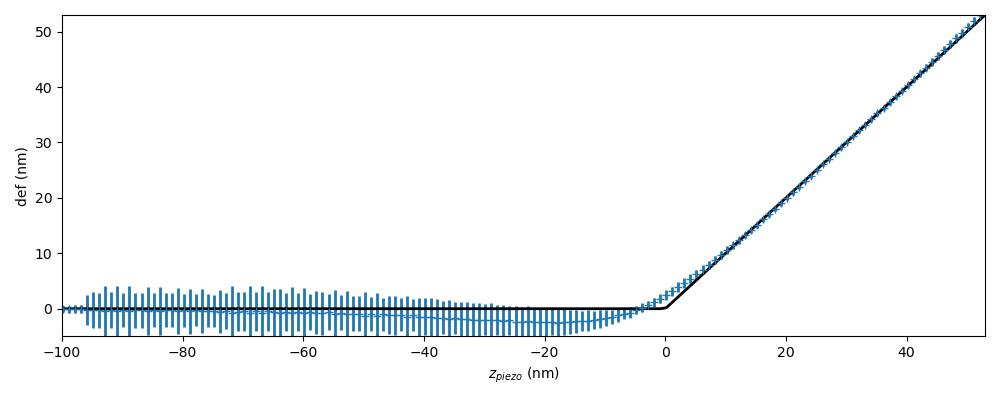
\includegraphics[width=\textwidth]{chapter7/ForceMaps/0.5mM/retract_df_zp_bin.jpg}
%    \caption{Retract df zp bin for 0.5mM concentration.}
%    \label{fig:retract_df_zp_bin_0.5mM}
%\end{figure}



\newpage
\subsubsection{10 mM approach}

The histogram shows a wide range of contact forces with a relatively large standard deviation. This suggests that at the 10 mM concentration, there is a significant variability in the forces measured across different sites of the surface during the approach phase. Interestingly, for some curves an attractive force was observed which is unlike the standard dataset. The attractive part of the curves are generally clustered towards the top of the heatmap suggesting that the surface has regions of varying repulsive forces. 

\begin{figure}[h!!!]
    \centering
    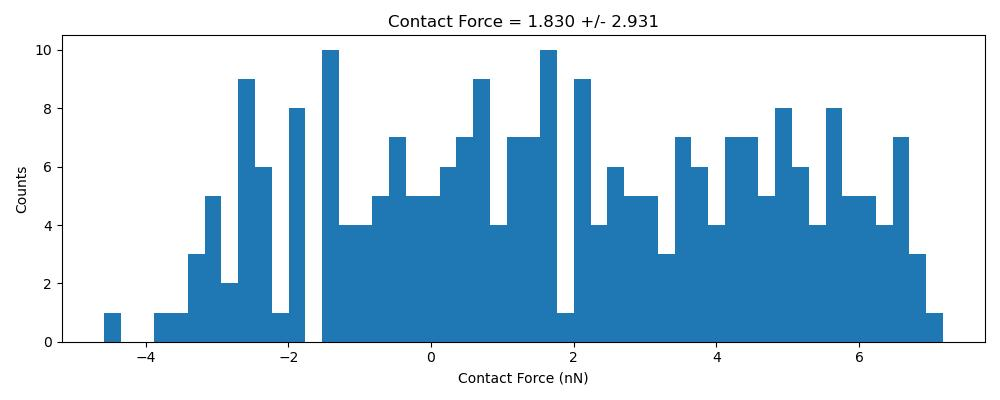
\includegraphics[width=0.7\textwidth]{chapter7/ForceMaps/10mM/approach_f_c_hist.jpg}
    \caption{Retract heatmap for 0.6 mM concentration.}
    \label{fig:appro_fc_10mM}
\end{figure}

% Approach heatmap
\begin{figure}[h!!!!!]
    \centering
    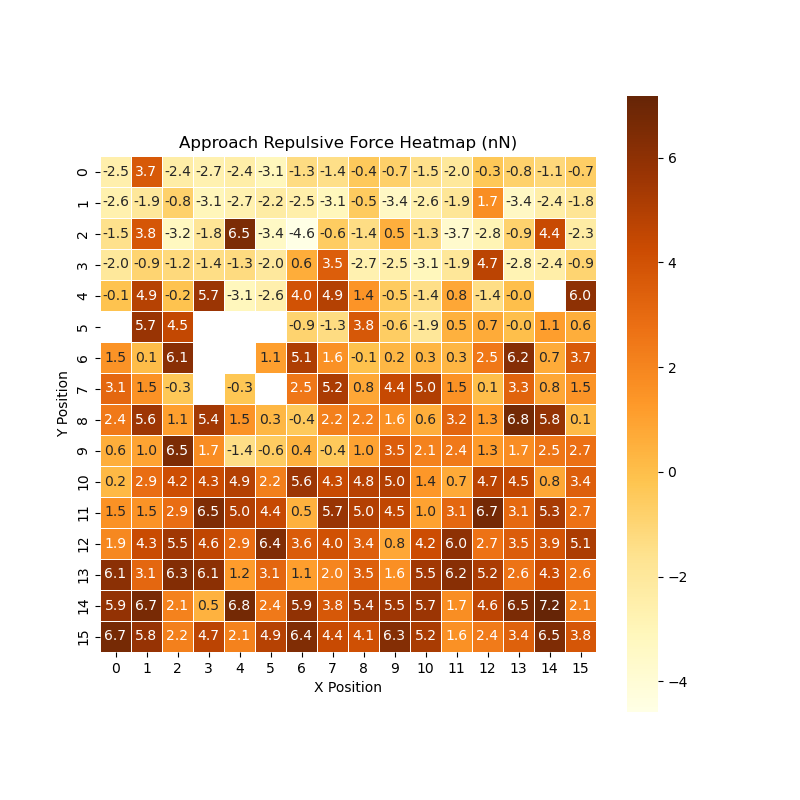
\includegraphics[width=0.75\textwidth]{chapter7/ForceMaps/10mM/Approach heatmap.png}
    \caption{Approach heatmap for 10 mM concentration.}
    \label{fig:approach_heatmap_10mM}
\end{figure}

\newpage 
\subsubsection{10 mM retract}

The retract portion of the curve is even more unusual with a consistent attractive force recorded at about 34 nN. This is unlike anything else seen in the dataset, so it is likely that the tip was contaminated or damaged, especially since the tip used was a reused one at the time.

\begin{figure}[h!!!]
    \centering
    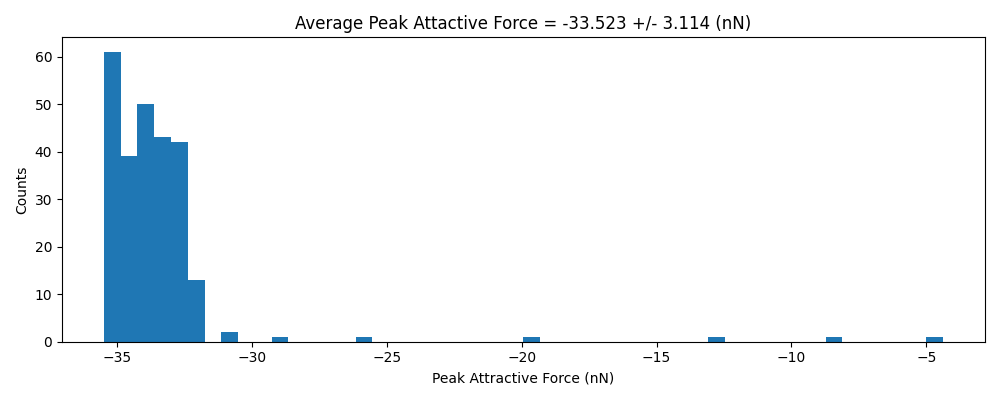
\includegraphics[width=0.79\textwidth]{chapter7/ForceMaps/10mM/contact_force_histogram.png}
    \caption{Retract heatmap for 0.6 mM concentration.}
    \label{fig:contfhist}
\end{figure}

\begin{figure}[h!]
\centering
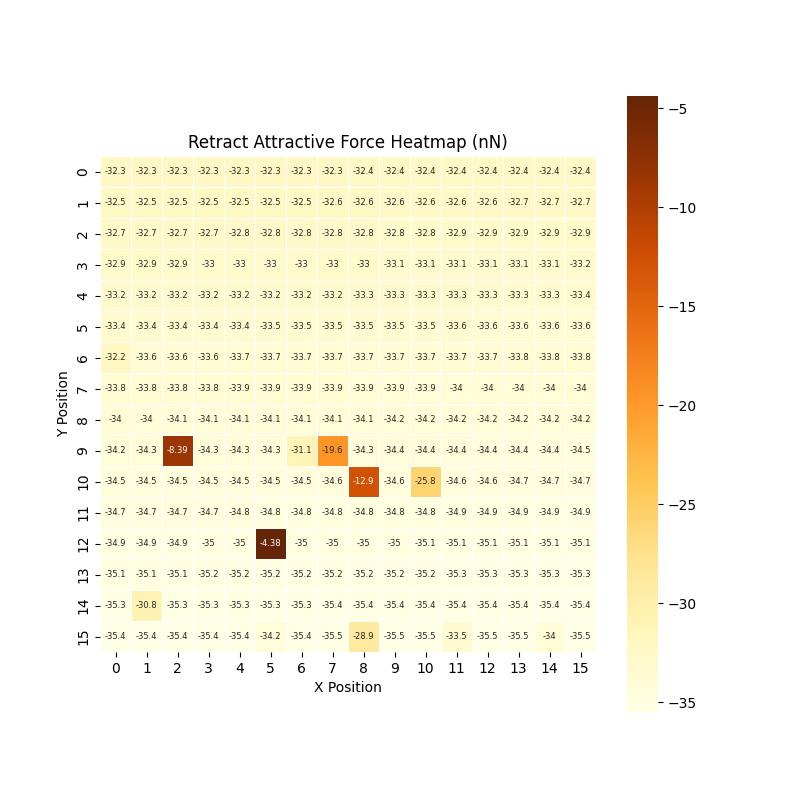
\includegraphics[width=0.7\textwidth]{chapter7/ForceMaps/10mM/Retract_heatmap.png}
\caption{Retract heatmap for 10 mM concentration.}
\label{fig:pHOverall}
\end{figure}

While the 10 mM results are ultimately suspicious, it does highlight the variability seen when interfacing a silica beat with the base of a borosilica petri dish. As to what could possibly cause these high degrees of variability, that leads us to the next chapter: the overall analysis of all of the data presented so far.
